\documentclass[a4paper,10pt]{article}
\usepackage[lmargin=2.0cm, rmargin=1.0cm,tmargin=3.5cm,bmargin=1.5cm]{geometry}
\usepackage{color,graphics}
\usepackage[export]{adjustbox}
\usepackage{lipsum}
\usepackage{multirow}
\usepackage{graphicx}
%\usepackage{lstlisting}

\usepackage{listings}
\usepackage[scaled=0.75]{helvet}

\begin{document}
\setcounter{secnumdepth}{-1} 

\begin{center}
\textbf{\LARGE Implement an application that stores big data in HBase using Hadoop.}
\end{center}

\raggedright Expt No: 8 \hfill \raggedleft May 27,2019 \\ 

\raggedright Author: Subalakshmi Shanthosi S (186001008) \par 


\section{Aim}
Implementation of storage in big data analytics using columnar database - HBase using Hadoop.

\section{Description}
\begin{enumerate}
	\item What is HBase?
	\begin{itemize}
		\item Apache HBase is a column-oriented key/value data store built to run on top of the Hadoop Distributed
		File System (HDFS).
		\item A non-relational (NoSQL) database that runs on top of HDFS.
		\item Provides real-time read/write access to those large datasets.
		\item Provides random, real time access to your data in Hadoop.
		\item Great choice to store multi-structured or sparse data. 
		\item Low latency storage .
		\item Versioned Database.
		\item Installation of HBase in standalone mode.
		
	\end{itemize}
	\item Advantages and Disadvantages of clustering methodologies: 
	\\
	$\bullet$ Advantages:
	\begin{itemize}
		\item Great for analytics in association with Hadoop MapReduce.
		\item It can handle very large volumes of data.
		\item Supports scaling out in coordination with Hadoop file system even on commodity hardware.
		\item Fault tolerance.
		\item License free.
		\item Very flexible on schema design/no fixed schema.
		\item Auto Sharding.
		\item Row-level atomicity, that is, the PUT operation will either write or fail.
	\end{itemize}
	$\bullet$ Disadvantages:
	\begin{itemize}
		\item Single point of failure (when only one HMaster is used).
		\item No transaction support.
		\item JOINs are handled in MapReduce layer rather than the database itself.
		\item Indexed and sorted only on key, but RDBMS can be indexed on some arbitrary field.
		\item No built-in authentication or permissions.
	\end{itemize}
\end{enumerate}
\newpage
\begin{table}[]
	\scalebox{0.6}{
		\begin{tabular}{|l|l|ll}
			\cline{1-2}
			\textbf{Column-oriented Database}                                                                                                                                              & \textbf{Row oriented Database}                                                                                                &  &  \\ \cline{1-2}
			\begin{tabular}[c]{@{}l@{}}When the situation comes to process and analytics we use this approach. Such as Online Analytical Processing\\  and it's applications.\end{tabular} & \begin{tabular}[c]{@{}l@{}}Online Transactional process such as banking and finance domains use this approach.\end{tabular} &  &  \\ \cline{1-2}
			The amount of data that can able to store in this model is very huge like in terms of petabytes & It is designed for a small number of rows and columns.                                                                        &  &  \\ \cline{1-2}
	\end{tabular}}
	\caption{Column-oriented vs Row-oriented storages
	}
	\label{tab:my-table}
\end{table}

\begin{figure}[h]
	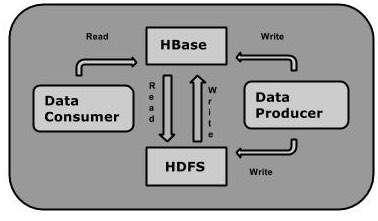
\includegraphics[scale=0.43,center]{0.jpg}
	\caption{Hadoop Random Access Databases.}
	\label{fig:01}
\end{figure}

\section{Procedure}

\begin{enumerate}
	\item Prepare a Virtual Machine Environment
	\item Install Java
	\item Install Hadoop
	\item Install HBase
\end{enumerate}	

\section{HBase Commands}
Write about HBase Commands
\begin{enumerate}
		\item \textbf{Create}:
			create a table in HBase with the specified name given according to the dictionary or specifications as per column family. In addition to this we can also pass some table-scope attributes 
			
			\begin{equation}
				 \textbf{create <tablename>, <columnfamilyname>}
			\end{equation}
		\item \textbf{Put}:			  
   		 It will put a celli'value' at defined or specified table or row or column.It will optionally coordinate time stamp.
			\begin{equation}
				\boldmath put <'tablename'>,<'rowname'>,<'columnvalue'>,<'value'>
			\end{equation}
		\item \textbf{Scan}:
		    We can pass several optional specifications to this scan command to get more information about the tables present in the system.Scanner specifications may include one or more of the following attributes.These are TIMERANGE, FILTER, TIMESTAMP, LIMIT, MAXLENGTH, COLUMNS, CACHE, STARTROW and STOPROW.
			\begin{equation}
				\boldmath scan <'tablename'>, {Optional parameters}
			\end{equation}

		\item \textbf{Get}:
		You will get a row or cell contents present in the table. In addition to that you can also add additional parameters to it like TIMESTAMP, TIMERANGE,VERSIONS, FILTERS, etc. to get a particular row or cell content. 
			\begin{equation}
				 \boldmath get <'tablename'>, <'rowname'>, {< Additional parameters>}
			\end{equation}
		\item \textbf{Disable}:
			 This command will start disabling the named table.f table needs to be deleted or dropped, it has to disable first.
			\begin{equation}
				\boldmath disable <tablename> 
			\end{equation}
		This command will disable all the tables matching the given regex.The implementation is same as delete command (Except adding regex for matching).Once the table gets disable the user can able to delete the table from HBase.Before delete or dropping table, it should be disabled first.
		    \begin{equation}
				\boldmath disable_all<"matching regex"> 
			\end{equation}
		\item \textbf{Drop}:
		    To delete the table present in HBase, first we have to disable it.    To drop the table present in HBase, first we have to disable it. So either table to drop or delete first the table should be disable using disable command.Here in above screenshot we are dropping table "education".Before execution of this command, it is necessary that you disable table "education".
		    \begin{equation}
				\boldmath drop <table name>
			\end{equation}
\end{enumerate}

\section{Output}

\begin{figure}[h]
	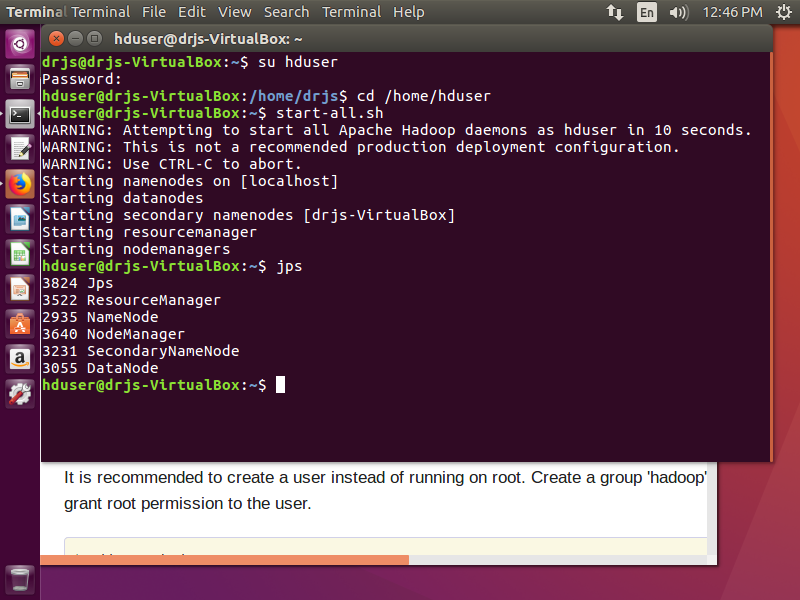
\includegraphics[scale=0.33,center]{1.png}
	\caption{Starting of Hadoop.}
	\label{fig:02}
\end{figure}

\begin{figure}[h]
	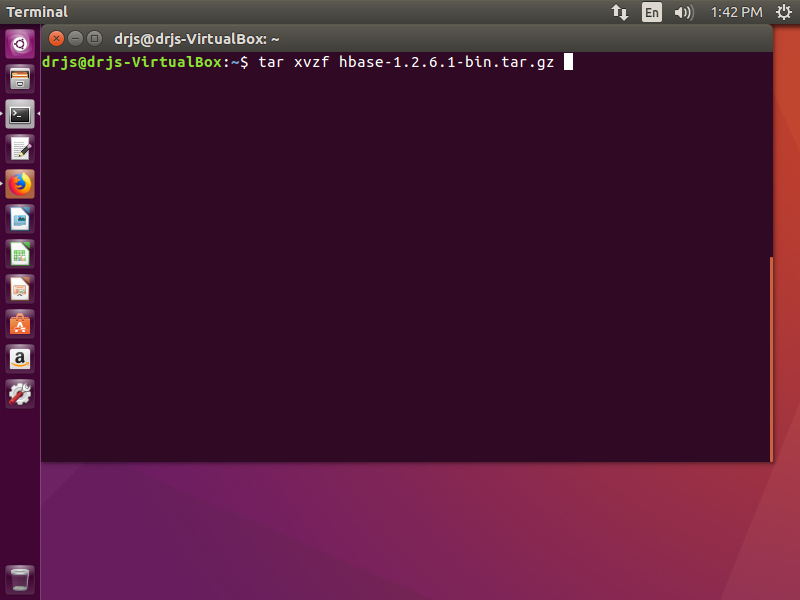
\includegraphics[scale=0.33,center]{2.png}
	\caption{Unzipping the hadoop file using tar command.}
	\label{fig:03}
\end{figure}	

\begin{figure}[h]
	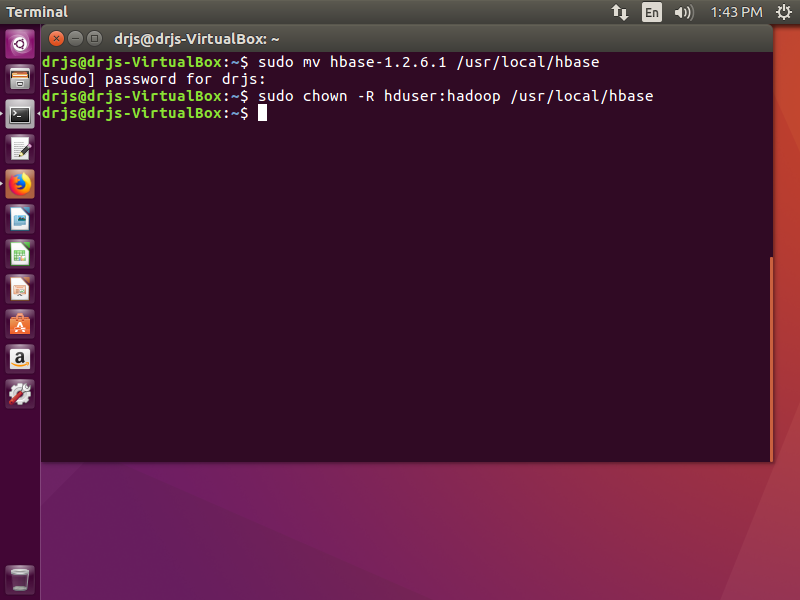
\includegraphics[scale=0.33,center]{3.png}
	\caption{Moving and changing the owner to /usr/local/hadoop.}
	\label{fig:04}
\end{figure}

\begin{figure}[h]
	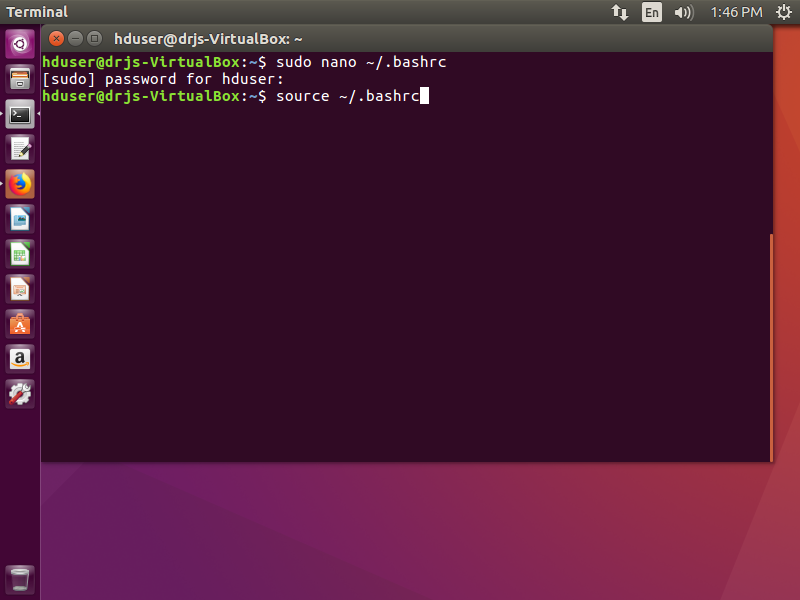
\includegraphics[scale=0.33,center]{4.png}
	\caption{Configuring bashrc.}
	\label{fig:05}
\end{figure}

\begin{figure}[h]
	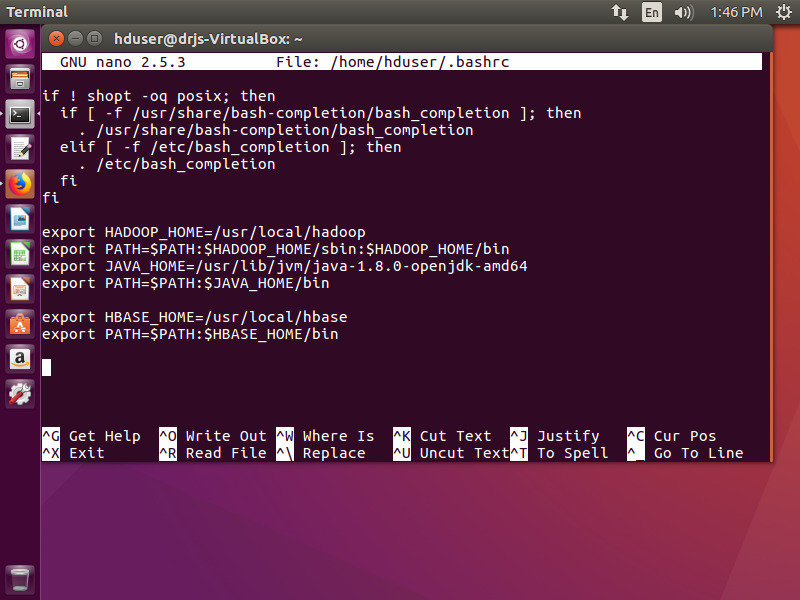
\includegraphics[scale=0.33,center]{5.png}
	\caption{Setting the hbase home and path.}
	\label{fig:06}
\end{figure}

\begin{figure}[h]
	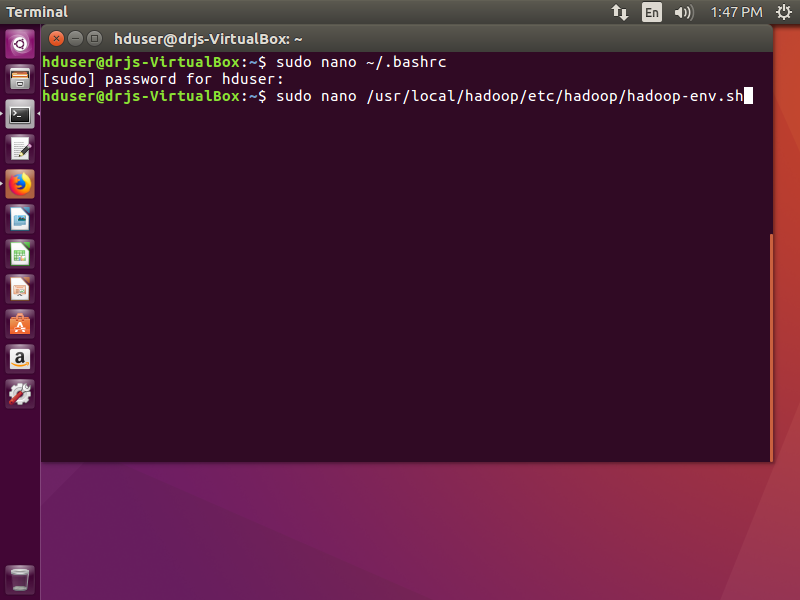
\includegraphics[scale=0.33,center]{6.png}
	\caption{Configuring hadoop-env.sh file.}
	\label{fig:07}
\end{figure}

\begin{figure}[h]
	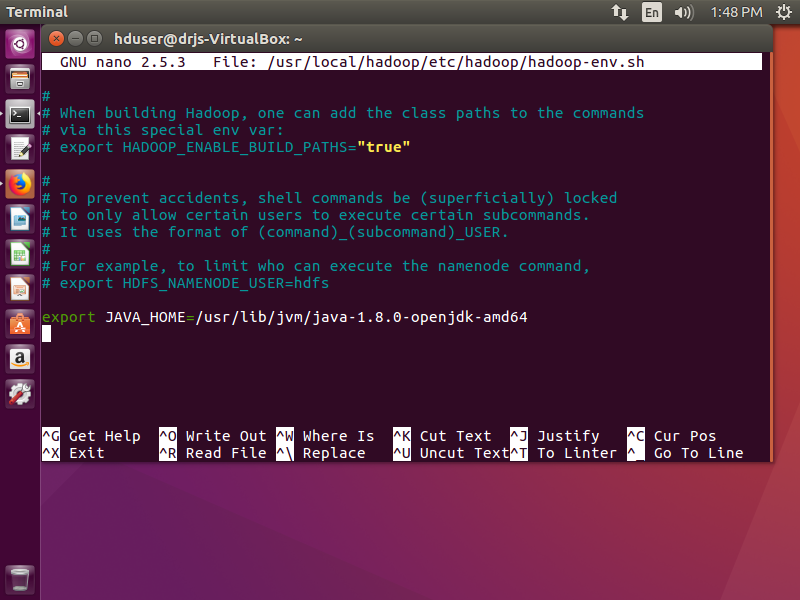
\includegraphics[scale=0.33,center]{7.png}
	\caption{Setting java path.}
	\label{fig:08}
\end{figure}

\begin{figure}[h]
	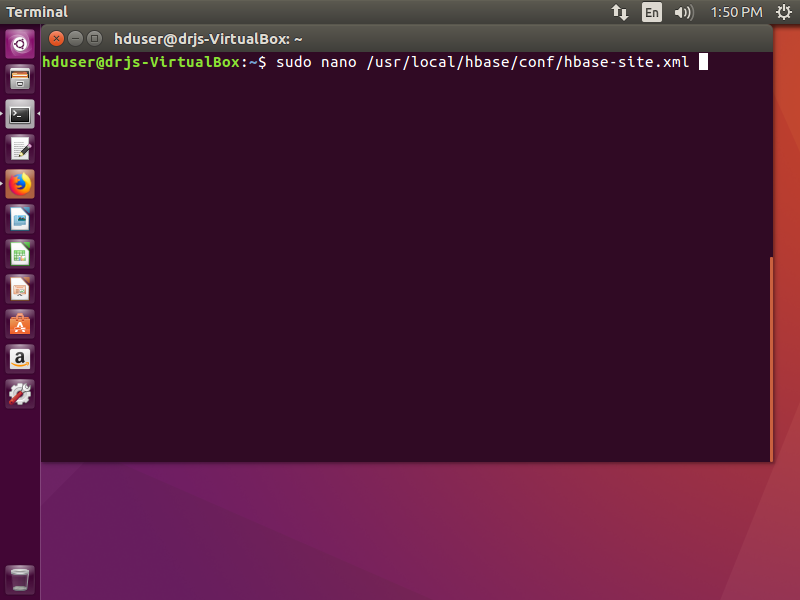
\includegraphics[scale=0.33,center]{8.png}
	\caption{Configuring hbase-site.xml file.}
	\label{fig:09}
\end{figure}

\begin{figure}[h]
	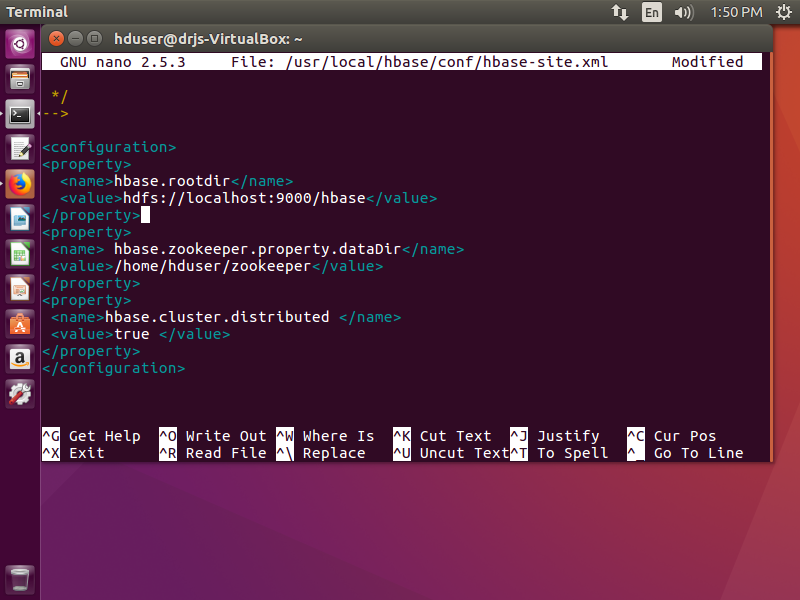
\includegraphics[scale=0.33,center]{9.png}
	\caption{hbase-site.xml.}
	\label{fig:10}
\end{figure}

\begin{figure}[h]
	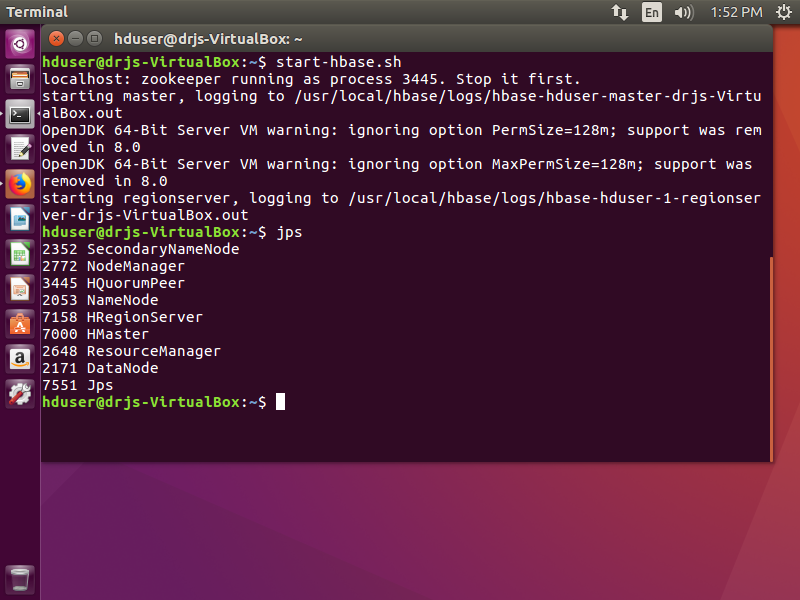
\includegraphics[scale=0.33,center]{10.png}
	\caption{Starting HBase.}
	\label{fig:11}
\end{figure}

\begin{figure}[h]
	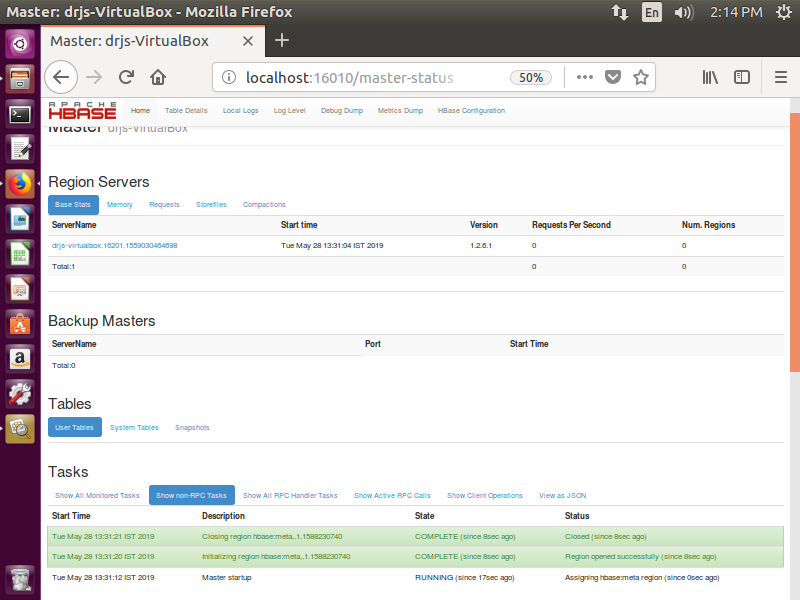
\includegraphics[scale=0.33,center]{19.png}
	\caption{Master status.}
	\label{fig:12}
\end{figure}

\begin{figure}[h]
	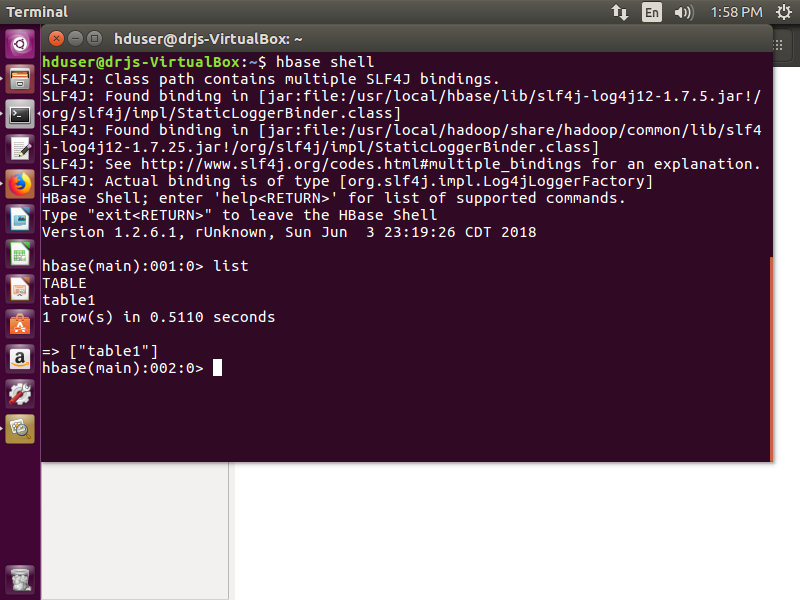
\includegraphics[scale=0.33,center]{11.png}
	\caption{hbase shell.}
	\label{fig:13}
\end{figure}

\begin{figure}[h]
	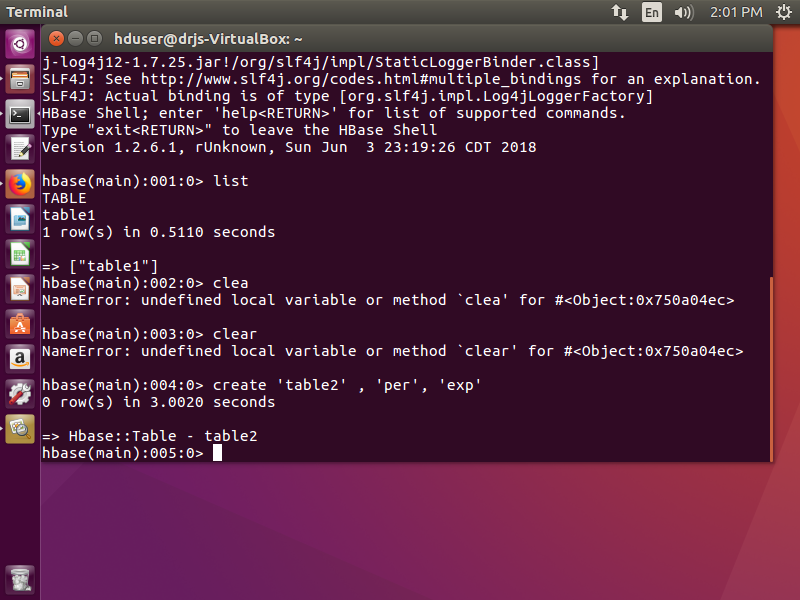
\includegraphics[scale=0.33,center]{12.png}
	\caption{Creation of table.}
	\label{fig:14}
\end{figure}

\begin{figure}[h]
	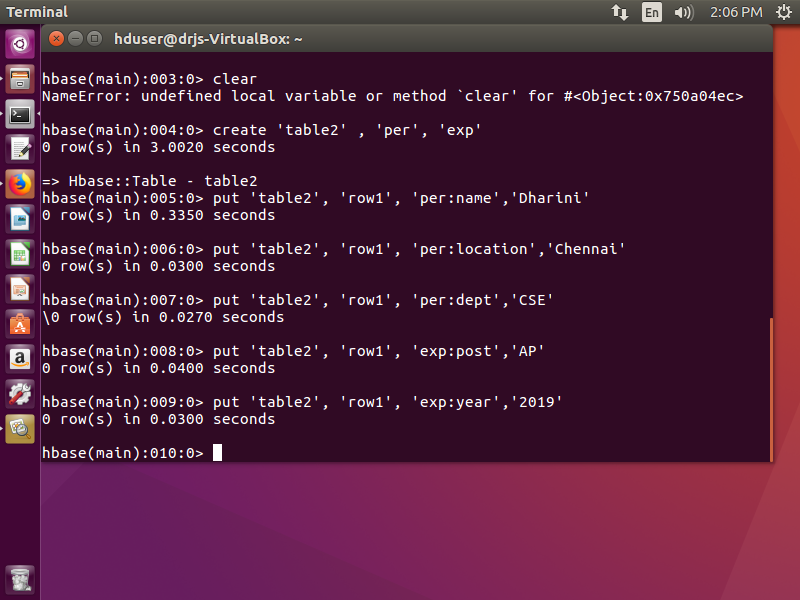
\includegraphics[scale=0.33,center]{13.png}
	\caption{Inserting rows using "put".}
	\label{fig:15}
\end{figure}

\begin{figure}[h]
	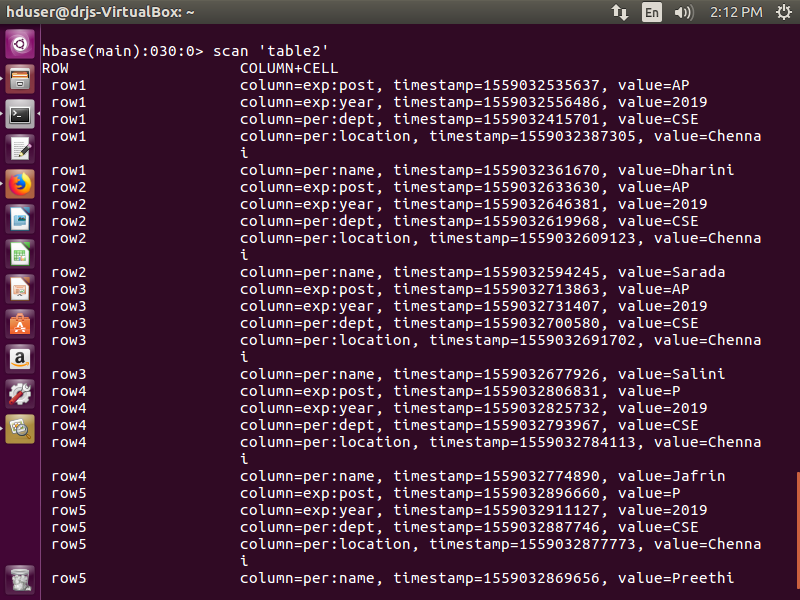
\includegraphics[scale=0.33,center]{17.png}
	\caption{Displaying the rows in table using "scan".}
	\label{fig:16}
\end{figure}

\begin{figure}[h]
	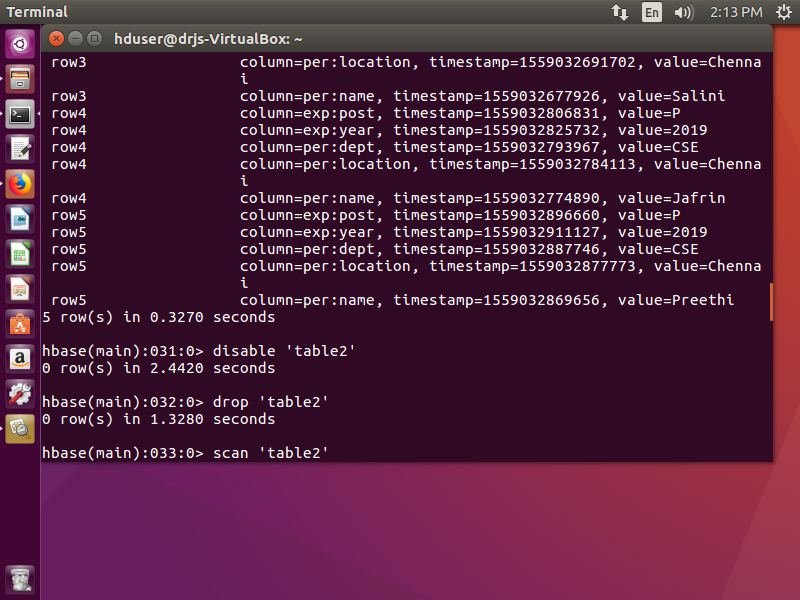
\includegraphics[scale=0.33,center]{18.png}
	\caption{Disabling and Dropping the table 2.}
	\label{fig:17}
\end{figure}
\begin{figure}[h]
	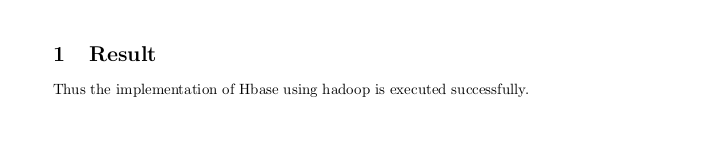
\includegraphics[scale=0.63]{result.png}
	\label{fig:18}
\end{figure}
\end{document}
